\subsection{Stereo Visualization}
\label{sec.stereo_visualization}

Let the distance of the eye to the screen, $d_{s}$, and the intra-ocular separation, $d_{io}$. Stereo view is enabled by translating the view off-center to the left by $d_{eye} = -d_{io}/2$,  and to the right by $d_{eye} = d_{io}/2$, as shown in Figure~\ref{fig.stereo_views}a. The view is split for left and right eyes using $M_{eye}$ in Equation~\ref{eq.stereo_view_matrix} combined with $M_{view}$.

\begin{equation}
\begin{aligned}
M_{eye} &= 
\begin{pmatrix} 
1 & 0 & 0 & d_{eye}\\
0 & 1 & 0 & 0\\
0 & 0 & 1 & 0\\
0 & 0 & 0 & 1\\
\end{pmatrix}
\end{aligned}
\label{eq.stereo_view_matrix}
\end{equation}

\begin{figure}[!hb]
\centering
\begin{tabular}{cc}
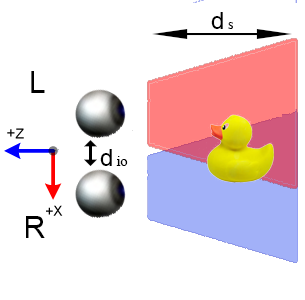
\includegraphics[width=0.35\linewidth,keepaspectratio=true]{figs/stereo_offset.png}
&
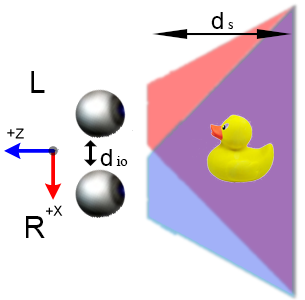
\includegraphics[width=0.35\linewidth,keepaspectratio=true]{figs/stereo_shear.png}
\\
(a)&(b)
\end{tabular}
\caption{Stereo views.}
\label{fig.stereo_views}
\end{figure}

Regarding the stereo technique to display the left and right views, adjustments in the horizontal, $s_x$, or vertical, $s_y$, scales are applied after the stereo view. In case of the modulation of the right and left views along time, there is no split and the view is fully displayed using  $s_x = s_y = 1$. In case of stereo split of the screen, each left and right views are scaled to half by $s_x = 2$, in case of vertical split, or by $s_y = 2$, in case of horizontal split. Both splits can be used to create the intertwined lines of right and left eye polarization.  

The convergence point is moved from $z=-\infty$ towards $+z$ by the shearing, as shown in Figure~\ref{fig.stereo_views}b, of the left and right projection frustum by $sh_z = d_{eye}/d_{s}$. The final stereo projection matrix, $M_{stereo}$, is a matrix scaled by $s_x$ and $s_y$, and sheared $sh_z$ in Equation~\ref{eq.stereo_proj_matrix}. The stereo pipeline is the sequence of transformations: $M_{stereo} \times M_{proj} \times M_{eye} \times M_{view}$.

\begin{equation}
\begin{aligned}
M_{stereo} &= 
\begin{pmatrix} 
s_x & 0 & 0 & 0\\
0 & s_y & 0 & 0\\
0 & 0   & 1 & 0\\
0 & 0   & 0 & 1\\
\end{pmatrix}
\begin{pmatrix} 
1 & 0 & sh_z & 0\\
0 & 1 & 0 & 0\\
0 & 0 & 1 & 0\\
0 & 0 & 0 & 1\\
\end{pmatrix}
\end{aligned}
\label{eq.stereo_proj_matrix}
\end{equation}

 